\section{Design}
I dette projekt er der valgt så vidt muligt at designe alle løsninger med analog elektronik. Derfor er det valgt at forforstærkeren bygges af commonemitter trin med uafkoblet emittermodstand. 
Argumentet for dette valg er at det er det eneste trin, blandt commonemitter, -base og -collector, hvis spændingsforstærkning ikke afhænger af transistorparametre. Da transistorparametre blandt andet er afhængige af den anvendte transistors temperatur er det en betragtelig styrke ikke at skulle tage højde for dem. Spændingsforstærkningen i commonemittertrinnet er dog kun uafhængig af transistorparametre så længe 



\begin{equation}
20 Pa \cdot 5 \frac{mV}{Pa} = 100 mV_{Peak}
\label{eq:mikrofonoutput}
\end{equation}

\subsection*{Kredsløb til mikrofon}

Mikrofonen som benyttes behøver skal, i følge databladet, have en supply spænding fra 1,5 til 10 V og en strøm på 0,5 mA. Desuden skal koblingskondensatorens størrelse være mellem 0,1-4,7$\mu$F. Kredsløbet til mikrofon vises på figur \ref{fig:mikrofonkreds}. 

\begin{figure}[h]
\centering
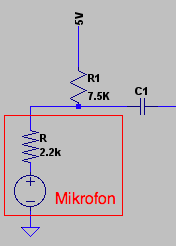
\includegraphics[scale=.6]{teknisk/forforstaerker/mikrofonkreds.png}
\caption{Supply kredsløb til mikrofonen}
\label{fig:mikrofonkreds}
\end{figure}

Spændingsfaldet over $R_1$ varierer sammen med mikrofonens output. Da strømmen gennem $R_1$ er lavest når spændingsfaldet er på sit minimum skal modstanden dimensioneres efter dette. Dermed bliver størrelse på $R_1$ i følge Ohms lov:

\begin{equation}
R_1 =  \frac{V_{R_1,min}}{I} = \frac{5-315 \cdot 10^{-3}}{0,5 \cdot 10^{-3}} = 9,37 k\Omega
\end{equation}

Koblingskondensatorens, C1, størrelse vil være afhængig af den modstand den kigger ind i og vil derfor blive dimensioneret i sammenhæng med forforstærkerkredsløbet \fixme{ref til forforstærkerkredsløbsdesign. Laaaangt ord.}

\subsection*{Kredsløbsdesign}

Hvad skal dette afsnit gøre?:
Forklare hvilke valg der er blevet truffet i designprocessen og hvorfor.



